\documentclass[a4paper,12pt]{article}

\usepackage[utf8]{inputenc}
\usepackage{polski}
\usepackage{fullpage}
\usepackage{hyperref}
\usepackage[pdftex]{graphicx} % Wsparcie dla obrazkow

\title{Wyznaczanie reprezentacji preferencji uniwersalych}
\author{Bartosz Górski \and Marcin Kaczyński \and Paweł Sokołowski}

\begin{document}

\maketitle

\section{Opis zadania} 

Szablon do wypełnienia. Jak ktoś chce napisać jakiś konkretny rozdział to niech się przy nim wpisze - może być w komentarzu. 
Jak nie to się później rozdzieli zadania.\\

Przykład wykorzystania bibliografii\cite{fst}. W bibliografii wpisy są z jakiegoś mojego wcześniejszego raportu, będą zmienione. Kompilacja:

\begin{itemize}
\item pdflatex raport (chyba musi być)
\item bibtex raport
\item pdflatex raport (x2)
\end{itemize}

Jak ktoś nie umie pisać w texie, to niech prześle plain text w notaniku.

\section{Założenia}
\section{Dane wejściowe i wyjściowe}
\section{Szczegóły implementacji}

Implementacja została przygotowana w języku C\# i działa na platformie .NET Framework 4.0. Implementacja związana z algorytmem została podzielona na 4 projekty: Algorithm, DAL, HashTree i pomocniczy projekt Common.\\

W projekcie Algorithm znajdują się wszystkie klasy i interfejsy w bezpośredni sposób związane z interfejsem. Projekt DAL zawiera implementacje dostępu do danych, a więc w tym przypadku parsowanie plików z danymi do postaci wykorzystywanej w algorytmie. W projekcie HashTree znalajdują się interfejsy i implementacja drzewa mieszającego. Projekt Common zawiera wspólne klasy wykorzystywane w pozostałych projektach. W projekcie Common znajdują się niemal jedynie obiekty DTO. Obiekty te same w sobie nie wykonują operacji, dlatego nie będą szczegółowo opisywane.\\

W celu zapewnienia elastyczności skorzystano w projekie ze wzorca Dependency Injection. Zgodnie z wzorcem, na implementację algorytmu składa się szereg interfejsów, których odpowiedzialności przestawiaja się następująco:\\

Za główny interfejs można uznać \textit{IAlgorithm}, a jego podstawowym zadaniem jest znajdowanie preferencji uniwersalnych. Interfejs jest implementowany przez klasy \textit{Generators} i \textit{ModifiedApriori}. Podstawowa różnica pomiędzy klasami polega na tym, że klasa Generators do obliczania minimalnych preferencji wykorzystuje informację o generatorach do odrzucania większej liczby zbiorów kandydujących. Obie implementacje operują na wierszach
typu \textit{Row}/\textit{SimpleRow}, które są odwzorowaniem danych w postaci wygodnej do prowadzenia obliczeń. Do znajdywania zbiorów kandydujących wykorzystywany jest interfejs \textit{ICandidatesGenerator}. Za znajdowanie podzbiorów wspieranych w transakcjach odpowiada \textit{IHashTree}. Wczytywanie danych odbywa się za pomocą \textit{IDataManager}, a konwersja wyników do postaci wygodnej dla użytkownika za pomocą \textit{IResultsConverter}.\\

Ogólnie przebieg działania całego algorytmu składa się z następujących kroków:

\begin{enumerate}
\item wczytanie i parsowanie danych,
\item wykonanie obliczeń,
\item parsowanie wyników do czytelnej postaci
\end{enumerate}

Wykonanie obliczeń (2) przebiega wg następującego schematu:\\

W kolejnych iteracjach znajdywane są nowe zbiory kandydujące, dla wszystkich zbiorów obliczane są dwa liczniki mówiące o tym jakie wsparcie mają te zbiory w klasie transakcji spełniających i nie spełniających relację. Aby zapewnić wydajne obliczanie wartości omawianych liczników, wykorzystywane jest drzewo mieszające tworzone w każdej iteracji dla zbioru kandydatów. Po obliczeniu liczników podejmowana jest decyzja o tym, czy dany kandydat
jest minimalnym wzorcem, czy należy go odrzucić lub analizować dalej. Na tym etapie (opcjonalnie) podejmowana jest decyzja czy któryś z podzbiorów danego zbioru kandydującego jest generatorem. Jeżeli tak, taki zbiór nie będzie analizowany dalej.

\section{Wyniki}

\subsection{Wyniki podstawowe}

\begin{figure}[h!]
\begin{center}
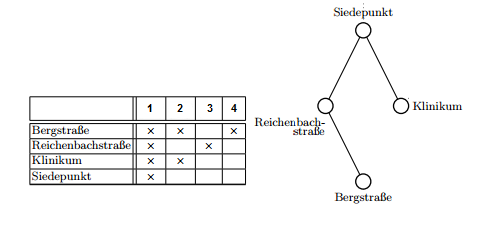
\includegraphics[width=\textwidth]{img/dane.png}
\caption{Dane podstawowe}
\label{dane_podstawowe}
\end{center}
\end{figure}

Na rysunku \ref{dane_podstawowe} przedstawiono tabelę z danymi i tabelę relacji w których pozostają klasy dla tych danych. Poniżej znajdują się szczegółowe wyniki dla tego zbioru.\\

Dla tego przypadku tworzone jest następujące mapowanie wartości atrybutów na liczby naturalne:\\

\begin{itemize}
\item 1 i 4 - vegetarian meal
\item 2 i 5 - non-vegetarian meal without pork
\item 3 i 6 - other meal
\item 4 i 8 - meal containing alcohol
\end{itemize}

Atrybuty 5, 6, 7 i 8 powstają w wyniku połączenia dwóch zbiorów.\\

W dalszej częśći tej sekcji dla skrócenia zapisów kandydaci będą opisywani trójką w postaci (0 - (12, 4)), gdzie pierwsza wartość jest indeksem atrybutu, a dwa kolejne to liczniki mówiące o wsparciu w klasach decyzyjnych.

\subsubsection{Relacja ścisła}

W przypadku gdy relacja ma zachodzić w sposób ścisły algorytm znajduje następujące minimalne wzorce kontrastowe:

\begin{enumerate}
\item (other meal) $=>$ (meal containing alcohol) \label{res1}
\item (non-vegetarian meal without pork, meal containing alcohol) $=>$ () \label{res2}
\item (other meal, meal containing alcohol) $=>$ () \label{res3}
\end{enumerate}

Przebieg algorytmu dla tego przypadku, przedstawia się następująco:\\

W pierwszej iteracji algorytm nie odnajduje żadnych wzorców. Kandydaci: (0 - (12, 4)), (4 - (12, 4)), (5 - (8, 0)), (6 - (4, 0)) są odrzucani,
a dalszej analizie podlegają kandydaci: (1 - (5, 3)), (2 - (2, 2)), (7 - (3, 1)), (3 - (3, 1)). Kandydaci 0 i 4 są odrzucani ponieważ zbiór pusty jest ich generatorem, a kandydaci 5 i 6 ponieważ relacja nie jest dla nich spełniona ani razu.\\

W drugiej iteracji algorytm znajduje minimalne wzorce (2, 7 - (0, 1)) mapowany na \ref{res1}, (1, 3 - (0, 0)) \ref{res2} oraz (2, 3 - (0, 0)) \ref{res3} do analizy pozostaje 1 kandydat (1, 7 - (1, 1)) z którego nie można już wygenerować kandydatów 3 elementowych, a kandydaci (1, 2 - (2, 2)) i (3, 7 - (1, 0)) są odrzucani.\\

W przypadku gdy nie wykorzystuje się własności związanej z generatorami, przebieg algorytmu wygląda następująco:\\

W pierwszej iteracji tylko dwóch kandydatów jest wykluczanych z dalszej analizy: (5 - (8, 0)), (6 - (4, 0)). W związku z tym w drugim kroku jest generowanych więcej kandydatów z których aż 11 podlega dalszej analizie: (0, 1 - (5, 3)), (0, 2 - (2, 2)), (0, 4 - (12, 4)), (1, 2 - (2, 2)), (1, 4 - (5, 3)), (2, 4 - (2, 2)), (0, 7 - (3, 1)), (1, 7 - (1, 1)), (4, 7 - (3, 1)), (0, 3 - (3, 1)), (3, 4 - (3, 1)). W kolejnym kroku 8 kandydatów o 3 elementach zostaje do dalszej analizy i dalej 2 kandydatów 4 elementowych.

\subsubsection{Relacja nie ścisła}

W przypadku gdy relacja ma zachodzić w sposób nie ścisły algorytm znajduje następujące minimalne wzorce kontrastowe:

\begin{enumerate}
\item (other meal, other meal) $=>$ ()
\item (other meal) $=>$ (meal containing alcohol)
\item (meal containing alcohol) $=>$ (meal containing alcohol)
\item (non-vegetarian meal without pork, meal containing alcohol) $=>$ ()
\item (other meal, meal containing alcohol) $=>$ ()
\item (non-vegetarian meal without pork) $=>$ (meal containing alcohol)
\item (other meal) $=>$ (meal containing alcohol)
\end{enumerate}

\subsubsection{Równoważność}

W przypadku gdy relacja ma zachodzić w sposób równoważny algorytm znajduje następujące minimalne wzorce kontrastowe:

\begin{enumerate}
\item (other meal, other meal) $=>$ ()
\item (meal containing alcohol) $=>$ (meal containing alcohol)
\item (non-vegetarian meal without pork, meal containing alcohol) $=>$ ()
\item (other meal, meal containing alcohol) $=>$ ()
\item (non-vegetarian meal without pork) $=>$ (meal containing alcohol)
\item (other meal) $=>$s (meal containing alcohol)
\end{enumerate}

\subsection{Wyniki dla złożonych danych}

A tutaj wyniki dla normalnych danych. Na pewno musi być zbiór z samochodami, ten który był na którymś lab.

\section{Wnioski}

\appendix
\section{Podręcznik użytkownika}

Do uruchomienia aplikacji wymagany jest zainstalowany .NET Framework 4.0. Nie jest konieczna instalacja dodatkowych programów, bibliotek lub komponentów.\\

Do obsługi algorytmu został przygotowany prosty graficzny interfejs, opierający
się na idei instalatora. W kolejnych krokach użytkownik wybiera kolejne dopuszczalne opcje i zatwierdza je klikając przycisk Next. Możliwe jest cofnięcie się do poprzedniego widoku za pomocą przycisku Prev. Kolejne widoki wyglądają następująco:

\begin{figure}[h!]
\begin{center}
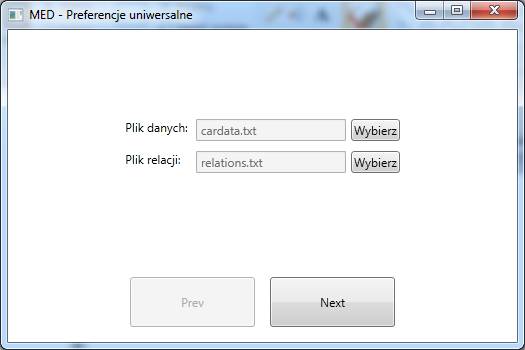
\includegraphics[width=\textwidth]{img/1.png}
\caption{Wybór plików z danymi}
\label{krok1}
\end{center}
\end{figure}

W kroku pierwszym\ref{krok1} należy wbrać pliki z danymi, klikając w przyciski Wybierz. Pliki wybiera się wykorzystując standardowy dialog wyboru plików z systemu Windows. Nie ma ograniczenia na rozszerzenie pliku.\\

Plik z danymi powinien być poprawnym pod względem budowy plikiem csv. W pliku powinny być kolejne wiersze w których w każdym znajduje się taka sama liczba kolumn oddzielonych określonym separatorem.\\

todo - słowo o postaci pliku z relacjami\\

\begin{figure}[h!]
\begin{center}
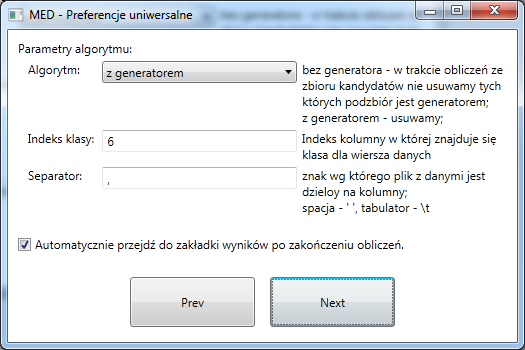
\includegraphics[width=\textwidth]{img/2.png}
\caption{Wybór parametrów}
\label{krok2}
\end{center}
\end{figure}

W kroku drugim\ref{krok2} należy wybrać parametry algorytmu. Dopuszczono wybór samego algorytmu - możliwe jest wykonanie algorytmu w wersji wykorzystującej oraz nie wykorzystującej faktu o podzbiorach będących generatorami.\\

W tym kroku należy również wybrać separator wykorzystywany w pliku danych, określić indeks kolumny która zawiera klasę do której przypisany jest dany wiersz, oraz określić rodzaj relacji na podstawie którego uzupełniane są dane w tabeli transakcji.\\

\begin{figure}[h!]
\begin{center}
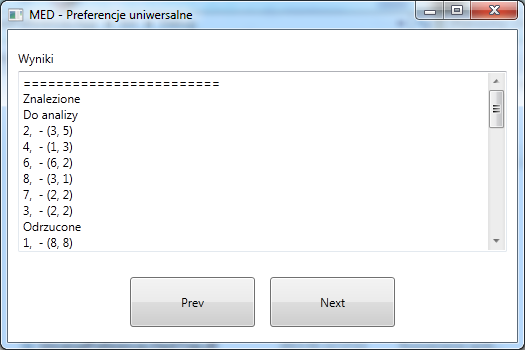
\includegraphics[width=\textwidth]{img/3.png}
\caption{Widok obliczeń}
\label{krok3}
\end{center}
\end{figure}

Krok trzeci\ref{krok3} to widok prezentowany w trakcie wykonywania obliczeń. W widoku wyświetlane są informacje diagnostyczne mówiące o tym które zbiory kandydujące zostały uznane za minimalne wzorce kontrastowe, które zostały odrzucone a które zostaną poddane dalszej analizie. Jeżeli w poprzednim kroku zaznaczono opcję Automatycznie przejdź do zakładki wyników po zakończeniu obliczeń, to po znalezieniu wszystkich wzorców program wyświetli widok wyników\ref{krok4}.\\

\begin{figure}[h!]
\begin{center}
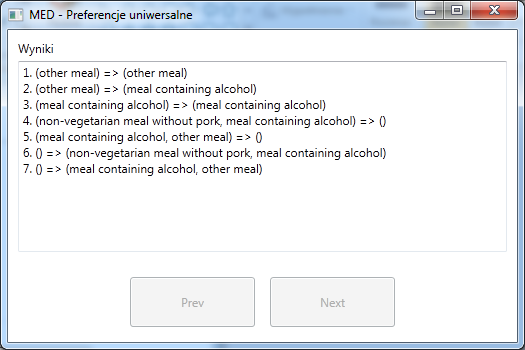
\includegraphics[width=\textwidth]{img/4.png}
\caption{Widok wyników}
\label{krok4}
\end{center}
\end{figure}

\bibliographystyle{plain}
\bibliography{bibliografia}

\end{document}
